\documentclass[letterpaper]{article}
\usepackage[utf8]{inputenc}
\usepackage[T1]{fontenc}
\usepackage[activeacute,spanish]{babel}
\usepackage[vmargin=4cm,tmargin=3cm,hmargin=2cm,letterpaper]{geometry}%
\usepackage{helvet}
\usepackage{amsmath,amsfonts,amssymb}
\usepackage{graphicx}
\usepackage{color}
\usepackage{xcolor}
\usepackage{verbatim}
\usepackage{tabls}
\usepackage{lastpage}
\usepackage{fancyhdr}
\usepackage{url}
\usepackage{listings}
\usepackage{hyperref}
%%%%%%%%%%%%%%%%%%%%%%%%%%%%%%%%%%%%%%%%%%%%%%%%%%%%%%%%%%%%%%%%%%%%%%%%%%%%%%%%%%%%%%%
\usepackage{tikz}
\usepackage{pgf}
\usepackage{pgffor}
\usepgfmodule{plot}
\usepackage{wrapfig}
\usetikzlibrary{arrows,decorations,snakes,backgrounds,fit,calc,through,scopes,positioning,automata,chains,er,fadings,calendar,matrix,mindmap,folding,patterns,petri,plothandlers,plotmarks,shadows,shapes,shapes.arrows,topaths,trees}

\lstset{% general command to set parameter(s)
%   basicstyle=\small,
  % print whole listing small
%   keywordstyle=\color{black}\bfseries\underbar,
  % underlined bold black keywords
%   identifierstyle=,
  % nothing happens
%   commentstyle=\color{white}, % white comments
%   stringstyle=\ttfamily,
  % typewriter type for strings
  showstringspaces=false}
  % no special string spaces

\pagestyle{fancy}
\color{black}
\fancyhead{}
\renewcommand{\headrule}{\hrule\vspace*{0.5mm}\rule{\linewidth}{0.8mm}}
\renewcommand{\familydefault}{\sfdefault}

%%%%%%%%%%%%%%%%%%%%%%%%%%%%%%%%%%%%%
\makeatletter
\define@key{PDF}{Movie}{\pdf@addtoks{#1}{Movie}}
\define@key{PDF}{Activation}{\pdf@addtoks{#1}{Activation}}
\newcommand{\moviewithpreview}[3]{% args: width, preview, movie
\pdfmark[{\includegraphics[width=#1]{#2}}]{%
pdfmark=/ANN,Subtype=/Movie,Movie=<< /F (#3) >>,%
Activation=<< /ShowControls true /Mode /Repeat >>}}
\newcommand{\movie}[3]{% args:width, height, movie
\pdfmark[{\hbox to #1 {\vbox to #2 { }}}]{%
pdfmark=/ANN,Subtype=/Movie,Movie=<< /F (#3) /Poster true >>,%
Activation=<< /ShowControls true /Mode /Repeat >>}}
\makeatother
%%%%%%%%%%%%%%%

\graphicspath{{./images/}}
\lhead{
\includegraphics[width=4cm]{pictures/ucr.png}}
\rhead{
\includegraphics[width=3cm]{pictures/eie.png}}
\chead{UNIVERSIDAD DE COSTA RICA\\FACULTAD DE INGENIERÍA\\ESCUELA DE INGENIERÍA ELÉCTRICA\\\textbf{ESTRUCTURAS ABSTRACTAS DE DATOS Y\\ ALGORITMOS PARA INGENIERÍA}\\IE-0217\\II CICLO 2014\\PROYECTO Final}

\lfoot{}%
\cfoot{}%
%\cfoot{\thepage\ de \pageref{LastPage}}%
\rfoot{}%

%%%%%%%%%%%%%%%%%%%%%%%%%%%%%%%%%%%%%%%%%%%%%%%%%%%%%%%%%%%%%%%%%%%%%%%%%%%%%%%%%%%%%%%%%%%%%%%%%%%%%%%%%%%%%%%
\newcommand{\uic}{blue} %user-input color
%%%%%%%%%%%%%%%%%%%%%%%%%%%%%%%%%%%%%%%%%%%%%%%%%%%%%%%%%%%%%%%%%%%%%%%%%%%%%%%%%%%%%%%%%%%%%%%%%%%%%%%%%%%%%%%%%%
\newcommand{\uim}{\_\_} %user-input marker
%%%%%%%%%%%%%%%%%%%%%%%%%%%%%%%%%%%%%%%%%%%%%%%%%%%%%%%%%%%%%%%%%%%%%%%%%%%%%%%%%%%%%%%%%%%%%%%%%%%%%%%%%%%%%%%%%%
\newcommand{\userinput}[1]{\textcolor{\uic}{\uim#1\uim}}


%%%%%%%%%%%%%%%%%%%%%%%%%%%%%%%%%%%%%%%%%%%%%%%%%%%%%%%%%%%%%%%%%%%%%%%%%%%%%%%%%%%%%%%%%%%%%%%%%%%%%%%%%%%%%%%%%%
\begin{document}\vspace*{2cm}
%%%%%%%%%%%%%%%%%%%%%%%%%%%%%%%%%%%%%%%%%%%%%%%%%%%%%%%%%%%%%%%%%%%%%%%%%%%%%%%%%%%%%%%%%%%%%%%%%%%%%%%%%%%%%%%%%%

%%%%%%%%%%%%%%%%%%%%%%%%%%%%%%%%%%%%%%%%%%%%%%%%%%%%%%%%%%%%%%%%%%%%%%%%%%%%%%%%%%%%%%%%%%%%%%%%%%%%%%%%%%%%%%%%%%
\begin{center}
\Huge
Comunicación por medio de Infrarrojo entre los robots humanoides NAO
\vspace*{1cm}
\end{center}

\noindent
\small\baselineskip=14pt
\textbf{Estudiantes:} Guido Armas González - José Pablo Ávila López - Lennon Núñez Meoño\\
\textbf{Carné:} B30647 - B30714 - B34943\\

\begin{center}
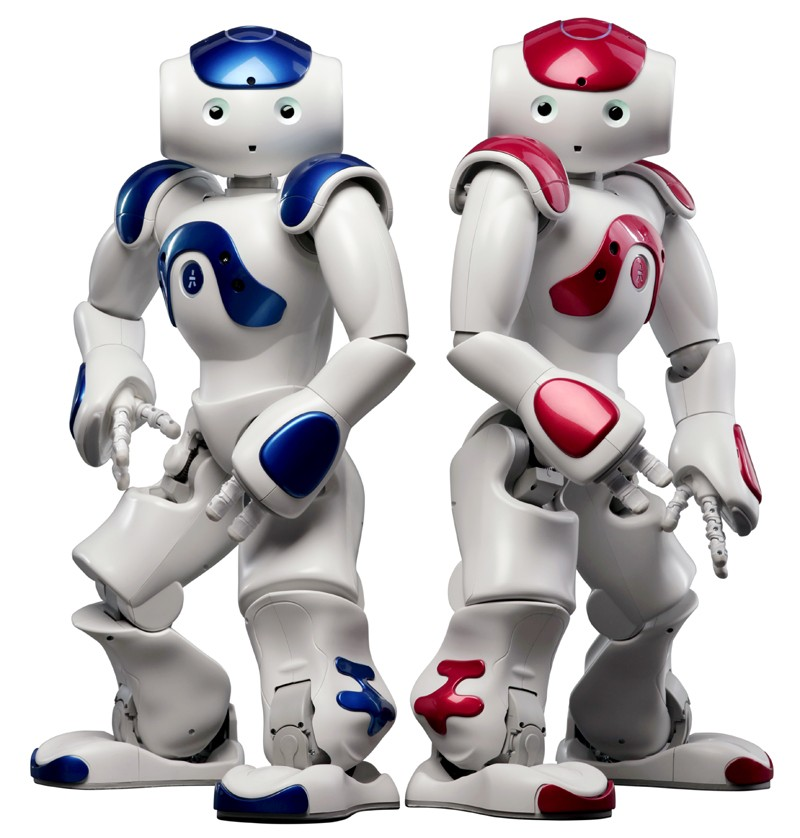
\includegraphics[width=4.5cm]{pictures/nao1.jpg}

\end{center}


%%%%%%%%%%%%%%%%%%%%%%%%%%%%%%%%%%%%%%%%%%%%%%%%%%%%%%%%%%%%%%%%%%%%%%%%%%%%%%%%%%%%%%%%%%%%%%%%%%%%%%%%%%%%%%%%%%
\section{Introducción}

Desde el comienzo de las adquisisiones por medio del ser humano, se ha visto la necesidad de crear sistemas de vgilancia que estén
al tanto de lo que sucede mientras uno no está un tanto o del todo enfocado en lo que sucede en cierto lugar. Con la llegada
de los dispositivos digitales (sensores, cámaras, entre otros) se ha visto una gran ventaja en cuanto a la creación de 
sistemas de vigilancia con la implementación de estos dispositivos, dentro de los que las cámaras de vigilancia han sido las de 
mayor auge. En la actualidad se intenta integrar lo que son sistemas robóticos a las actividades diarias del ser humano, o bien, a 
sustituir al humano de esos quehaceres, los sistemas de viglancia no están fuera de este cambio, se intenta crear sistemas de 
detección con reacciones mecanizadas de acuerdo a lo que el usuario desee.
\\ Los robots NAO nos ofrecen una opción de integración a estos sistemas, ya que incluyen sensores y cámaras en un ''empaquetado''
humanoide del que se puede sacar provecho. Por medio del proyecto en desarrollo se intenta crear un sistema de vigilancia
por medio de la implementación del módulo de comunicación por infrarrojo en interacción con la gama de posibilidades
que los motores, sensores y cámaras nos otorgan, creando una red a través de los NAO por la que se comuniquen la información
que cada uno de ellos obtenga en su zona de vigilancia, por ejemplo. Esta y otras ideas se tratarán de desarrollar a lo largo
del estudio del módulo de comunicación por infrarrojo con el enfoque en crear el sistema integrado de seguridad NAO.
%%%%%%%%%%%%%%%%%%%%%%%%%%%%%%%%%%%%%%%%%%%%%%%%%%%%%%%%%%%%%%%%%%%%%%%%%%%%%%%%%%%%%%%%%%%%%%%%%%%%%%%%%%%%%%%%%%
\section{Objetivos}

\subsection{Objetivo General}

Desarrollar un módulo para los dispositivos Nao H25 en C++ o python para la implementación de su sensor de Infrarojo en un sistema de vigilancia. 

\subsection{Objetivos Específicos}

Los objetivos específicos son:\\

\begin{enumerate}

\item Comprender el uso del módulo del sensor infrarojo del Nao.
\item Conocer los alcances del sensor Infrarojo.
\item Crear una librería en C++ o python con sus respectivos métodos para la comunicación y traspaso de información entre robots y computadoras utilizando el módulo de infrarojo.
\item Concretar una implementación del módulo infrarojo para un sistema de vigilancia con dispositivos Naos con funciones añadidas utilizando los demás módulos del robot.

\end{enumerate}
%%%%%%%%%%%%%%%%%%%%%%%%%%%%%%%%%%%%%%%%%%%%%%%%%%%%%%%%%%%%%%%%%%%%%%%%%%%%%%%%%%%%%%%%%%%%%%%%%%%%%%%%%%%%%%%%%%

\section{Justificación}

La presente investigación tiene como fin indagar sobre el módulo de infrarrojo del NAOqi y a su vez implementarlo con el fin de potenciar el uso de estos robots como una herramienta útil en la vida cotidiana, o sea, el desarrollo de aplicaciones basados en la comunicación por infrarrojo de los robots y con otros dispositivos soportados por este medio de comunicación. Una gran ventaja del uso del infrarrojo es el hecho de que es una manera muy común de recibir información en aparatos domésticos, lo cual brinda una gran gama de posibles aplicaciones a tareas cotidianas. 
\\ Otro de los motivos para llevar a cabo este proyecto es el de innovar en el uso del módulo infrarrojo en el PRIS-Lab, ya que es un tema que casi no se ha trabajado en el laboratorio, por lo cual se puede desarrollar este tema para ampliar la gama de aplicaciones en las que se usan los NAO y colaborar con alguna documentación a futuros proyectos que deseen abarcar distintos puntos de trabajo con la librería a estudiar para seguir la investigación y desarrollo de esta importante librería.  

%%%%%%%%%%%%%%%%%%%%%%%%%%%%%%%%%%%%%%%%%%%%%%%%%%%%%%%%%%%%%%%%%%%%%%%%%%%%%%%%%%%%%%%%%%%%%%%%%%%%%%%%%%%%%%%%%
\section{Metodología}

Se comprenderá el módulo ALInfrared y se utilizará para conocer sus limitaciones y alcances. Seguidamente se creará una librerá que necesitará de este módulo para enviar datos mediante los sensores infrarrojos entre los robots.
\\ Se buscará la interconexión de esta librería con otros módulos del Nao e intentar hacer su aplicación lo más fácil posible. Una vez obtenidos estos resultados se desarrollará un sistema de vigilancia de dos o más Naos que sean capaces de identificar un objeto (actividad sospechosa) y mediante el infrarojo enviarle un dato a otro robot empezando con un sistema binario, y se le añadiran funciones según avance el proyecto.


%%%%%%%%%%%%%%%%%%%%%%%%%%%%%%%%%%%%%%%%%%%%%%%%%%%%%%%%%%%%%%%%%%%%%%%%%%%%%%%%%%%%%%%%%%%%%%%%%%%%%%%%%%%%%%%%%%
\section{Desarrollo del Pryecto}
\subsection{Generalidades del código para NAOs en c++ con qibuild}
Antes de poder correr código remotamente en los NAO es necesario estar seguros de que se posee en el ordenador las carpetas necesarias para la compilación e importación de los módulos de NAO a utilizar.
Lo primero que se debe tener es la carpeta SDK oficial que se obtiene de Aldebaran, carpeta que contiene todos los módulos necesarios. Luego de que se tiene esta información, uno de los métodos de correr código en los NAO es por medio del qibuild, encargado de crear proyectos localmente por medio de los cuales se puede correr código remotamente en los NAO. Para obtener qibuild se corre el comando "sudo apt-get install qibuild".\\
Una vez obtenido qibuild y la carpeta SDK, iniciamos qibuild con el comando "qibuild init". Luego creamos la zona de trabajo de qibuild, denominados toolchains, por medio de " qibuild create \_ nombre del toolchain\_  \_ ubicación en la que se creará el toolchain\_   - -default". El --default creará el toolchain con las características predeterminadas. Una vez creado el toolchain es posible compilar código que se agregue en la dirección establecida. \\
Para poder compilar código con qibuild es necesario tener el documento .cpp (para el caso de c $++$) y un archivo CMakeList.txt en el cual se inlcuyen los comandos de qibuild para generar el ejecutable e incluir las librerías bases para el mismo. Acontinuación un ejemplo del CMakeList:\\
"cmake\_ minimum\_ required(VERSION 2.8)\\
project(infra)\\
\\
find\_ package(qibuild)\\
\\
\# Create a executable named infra\\
\# with the source file: main.cpp\\
\\
\# working file\\
qi\_ create\_ bin(infrarred "infrarred.cpp")\\
qi\_ use\_ lib(infrarred ALCOMMON ALVISION OPENCV2\_ CORE OPENCV2\_ HIGHGUI)\\
\\
\# Add a simple test:\\
enable\_ testing()\\
qi\_ create\_ test(test\_ infra "test.cpp")"\\

Con estos dos archivos es suficiente para poder crear un ejecutable. Usamos los comandos "qibuild configure -c \_ nombre del toolchain\_" que se encarga de asegurarse que el toolchain esté bien configurado antes de compilar el proyecto, luego se usa "qibuild make -c \_ nmbre del toolchain\_" que se encarga de compilar y generar los ejecutables según las instrucciones del CMakeList.\\
El archivo .cpp debe incluir todos los módulos que se usaran pertenecientes al SDK, si algún módulo no se encuentra en el SDK no podrá ser importado y por ende no podrá usarse, he ahí la importancia del SDK. Cada módulo tiene sus propias funciones relacionadas al nombre que reciben, por ejemplo ALInfrared contiene todas las funciones relacionadas al uso del infrarrojo del NAO, así como ALMemory contiene información perteneciente a accesos a memoria y variables del robot, ALAudioPlayer se encarga de temas relacionados a la reproducción y grabado de audio, etc. \\
A pesar de tener funcionalidades diferentes, tienen en común el llamado e implementación. Para poder tener acceso a los métodos de cada módulo es necesario crear una instancia de la siguiente manera\\
"AL::\_ módulo\_ \_ nombre de la instancia \_(argv[1], 9559)"\\
El argv[1] hace referencia a la dirección IP que se envió al ejecutable para correrlo remotamente, y el 9559 apunta al puerto de conexión, este valor es predeterminado para los NAO con el número correspondiente. Luego de la instancia se hacen los llamados a los distintos métodos heredados del módulo: "\_ nombre de la instancia\_ .\_ método a invocar\_ (\_ parámetros que recibe\_)"\\
De este modo se trabaja cada función que se desee, para cada módulo importado es necesaria la instancia, de otro modo no se puede acceder a sus métodos.\\
Para poder correr el ejecutable de manera remota es necesario que el código del archivo .cpp tenga el siguiente encabezado para iniciar el main:\\
"int main(int argc, char* argv[]) \\
\\
	//argv[1] contiene el IP del NAO al que se le enviará el código remotamente\\
\\
  if(argc != 2)\\
    std::cerr \< \< "Wrong number of arguments!" \< \< std::endl;\\
    std::cerr \< \< "Usage: infrared NAO\_ IP" \< \< std::endl;\\
    exit(2);\\
  "\\
En consola se debe introducir "\_ ejecutable a correr\_  \_ IP del NAO al que se desea en viar el código de manera remota\_ ".\\
El ejecutable se genera dentro de la carpeta del proyecto correspondiente en el directorio "bin", en la cual se almacenan todos los ejecutables que el CMakeList tiene para crear.\\

\subsection{Uso del Infrarrojo}
\subsubsection{Características Generales}
\begin{itemize}
\item Ángulo de recepción de $+\-$60 grados partiendo desde el centro de la cabeza del NAO
\item Distancia de aproximadamente 1m entre los sensores de un NAO y el otro
\item Longitud de onda de 940nm
\item Intensidad de 80 mW/sr
\end{itemize}

\subsubsection{Limitaciones}
Dentro de las limitaciones principales está el mismo rango de la angulación de recepción del infrarrojo, ya que conforme nos acercamos a los límites aumenta la probabilidad de que no se reciban datos. Además, si aumentamos la distancia de separación entre un NAO y otro es más dificil que el receptor capte la información transmitida hasta el punto en que no es capaz de recibir dato alguno. Estas cualidades hacen que para que se de una correcta transmisión de información por medio del infrarrojo los NAO tengan que estar "viéndose" prácticamente de frente a una corta distancia el uno del otro.\\

\subsubsection{Aplicaciones}
Mediante el uso del módulo infrarrojo del naoqi, es posible hacer que dos o mas robots interactúen. Esto permite que se puedan dividir las tareas con el fin de llevar a cabo la resolución de problemas de manera conjunta y así ser mas eficientes y veloces en su implementación\\
La mayoría de aplicaciones para este tipo de comunicación requieren de varios robots NAO, con el fin de abarcar mas áreas del espacio en el que se trabaja y realizar labores de manera integral. Por ejemplo, en situaciones de emergencia, los robots NAO que son utilizados dentro de un edificio pueden comunicarse mediante transmisión por infrarrojo con elementos del exterior y realizar un diagnóstico de la situación para enviarla. \\
También, otras aplicaciones pueden tener incursión en lugares como hospitales, al usar los robots como "enfermeros" que reporten si existe alguna anomalía con el paciente 

\section{Referencias}

\begin{enumerate}
\item Aldebaran-Robotics., \textit{NAO Software 1.14.5 documentation}, Recuperado de \href{https://community.aldebaran-robotics.com/doc/1-14/index.html#}{Nao documentation home}, 2012.
\item Aldebaran-Robotics., \textit{NALInfrared documentation}, Recuperado de \href{http://doc.aldebaran.com/1-14/naoqi/sensors/alinfrared.html#alinfrared}{Infrared overview}, 2012.
\end{enumerate}
	
\end{document}

